
\documentclass[12pt]{article}
\usepackage{amsmath}
\DeclareMathOperator*{\argmin}{arg\,min} % thin space, limits underneath in displays
\DeclareMathOperator*{\argmax}{arg\,max} % thin space, limits underneath in displays
\newtheorem{thm}{Theorem}
\usepackage{amssymb}
\usepackage{amsfonts}
\usepackage{mathrsfs}
\usepackage{bm}
\usepackage{indentfirst}
\setlength{\parindent}{0em}
\usepackage[margin=1in]{geometry}
\usepackage{graphicx}
\usepackage{setspace}
\doublespacing
\usepackage[flushleft]{threeparttable}
\usepackage{booktabs,caption}
\usepackage{float}
\usepackage{graphicx}
\usepackage[sort,comma]{natbib}
\usepackage[hidelinks]{hyperref}

\usepackage{import}
\usepackage{xifthen}
\usepackage{pdfpages}
\usepackage{transparent}

\newcommand{\incfig}[1]{%
\def\svgwidth{\columnwidth}
\import{./figures/}{#1.pdf_tex}
}




\title{}
\author{}
\date{}


\begin{document}



\section{Unemployment}

{\textbf {DEF:}} Unemployment occurs when a worker who is not currently employed is 
searching for a job without success.\\










{\textbf {Three types of unemployment:}} structural, frictional, and cyclical.

Structural and frictional unemployment occur even when the economy is healthy and
growing. Hence, {\textbf {structural and frictional unemployment are often called
natural unemployment.}}


\subsection{Structural Unemployment}
The transformation of modern economy has brought new jobs but also requires different
skills. Some old-fashioned jobs become obsolete, and lead to some unemployment.\\
Joseph Schumpeter coined the term {\textbf {creative destruction}} to describe this 
process of evolution.\\
{\textbf {Creative destruction}} occurs when the introduction of new products and 
technologies leads to the end of other industries and jobs.

{\textbf {Structural unemployment}} is caused by changes in the industrial make-up
of the economy.


{\textbf {Structural unemployment}} cannot be eliminated, but it can be reduced in a
number of ways.
\begin{enumerate}
\item workers must often retrain, relocate, or change their expectations in some way
		before they can work elsewhere.
\item Government policies: job training programs, relocation subsidies.
\end{enumerate}













\subsection{Frictional Unemployment and Job Search}

DEF: The unemployment caused by the time it takes workers to search for a job.


{\textbf {Reasons for unemployment:}}
\begin{enumerate}
\item Government policy
\item Information (Frictional unemployment)
\item Change in demand or improvement in technology (Structural unemployment)
\item Wage rigidity (Structural unemployment)
\item Recession (Cyclical unemployment)
\end{enumerate}


\subsubsection{Factors affect frictional unemployment}
Any factors that shorten job searches also decrease frictional unemployment, e.g., 
Internet.


Government disseminates job information can reduce the time of job finding.


\subsection{Government policy}
Government disseminates job information can reduce the time of job finding.

{\textbf {Government unemployment insurance}} program prolongs the time of job finding 
because unemployed individuals are less stressful when they receive the benefit from 
unemployment insurance. They will ignore unattractive job opportunities.

{\textbf {Regulations on hiring and firing}}:\\
1. Regulations on hiring: who can and must be interviewed, paperwork, and additional
tax documents.

2. Regulations on firing: mandatory severance pay, government fines, written
justification.

These policies secure employees but raise cost for firms. It is more difficult to 
hire employees, and more potential cost to retain them. Firms will spend more time
when they are making hiring decision. This increases the {\textbf {frictional 
unemployment}}.









\subsection{Wage Rigidity}
{\textbf {DEF:}} the failure of wages to adjust to a level at which labor supply 
equals labor demand. Sometimes the real wage is stuck above the market-clearing level
(stick wage).


\begin{figure}[H]
\center{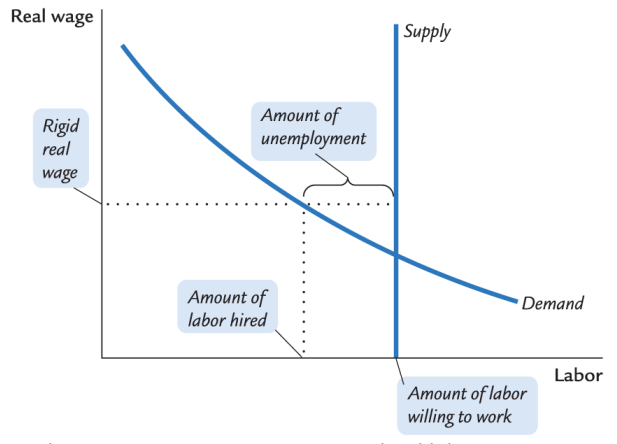
\includegraphics[scale =.5 ]  {figures/wage_rigidity.png}}
\end{figure}


When the real wage is above the equilibrium level, there is a excess of supply in 
labor. When firms fail to reduce the real wage, for whatever reason, it reduces the 
rate of job finding, $ f $, and raises the level of unemployment. 
The unemployment resulting from wage rigidity and job rationing is called
{\textbf {structural unemployment}} (There is a mismatch between the number of people
who want to work and the number of jobs that are available.)


\subsubsection{Three causes of wage rigidity}
They are {\textbf {minimum-wage laws}}, {\textbf {the monopoly power of unions}}, and
{\textbf {efficiency wages}}.\\


{\textbf {Minimum-wage Laws:}}
Minimum wage targeting on teenagers and low skill worker. However, firms will prefer
to hire more experienced worker especially when the cost of labor is increased under
the minimum wage police. More low-skilled workers is laid off. (Recall the minimum
wage, price floor, in microeconomics.)\\


{\textbf {Unions and collective bargaining:}}
\\



{\textbf {Efficiency wages:}}\\
The efficiency wage theories hold that high wages make workers more productive.\\
One theory, more relevant in poor countries, holds that wages influence nutrition,
then affect productivity.

A second theory, more relevant for developed countries, holds that high wages reduce 
labor turnover .

A third theory, quality of firm's workforce depends on the wage (adverse selection).


A fourth, high wage improves worker effort (moral hazard).






\subsection{Cyclical Unemployment}
It is caused by recessions, or economic downturns.





\subsection{The natural rate of unemployment}
The natural rate of unemployment, $ u^{*} $, is the typical unemployment rate
(considering structural and frictional unemployment)
that occurs when the economy is growing normally. The $ u^{*} $ in the US is between
$ 4\% $ and $ 5\% $.


When the unemployment rate is equal to the natural rate, the output level produced by
the economy is called {\textbf {full-employment output}}, $ Y^{*} $. It is also called 
potential output or potential GDP.\\



Healthy economy:
\begin{equation*}
u = u^{*}, \quad Y = Y^{*}, \text{ cyclical unemployment} = 0
\end{equation*}
Recession:
\begin{equation*}
u > u^{*}, \quad Y < Y^{*}, \text{ cyclical unemployment } > 0
\end{equation*}
Exceptional Expansion:
\begin{equation*}
u < u^{*}, \quad Y > Y^{*}, \text{ cyclical unemployment } < 0
\end{equation*}

It is possible for $ u > u^{*} $. It can happen temporarily. Demand for output might
be so high.



\subsection{Unemployment Rate}
The unemployment rate is released monthly.


{\textbf {Labor force:}} People who are employed or actively seeking work and are
work-eligible. A jobless person has not sought a job in four weeks is not counted 
in the labor force.



\begin{figure}[ht]
    \centering
    \incfig{structure}
    \label{fig:structure}
\end{figure}


\begin{align*}
\text{ Unemployment rate } &= \frac{U}{L}  \\
\text{ Labor participation rate } &= \frac{L}{\text{ work-Eligible }} 
\end{align*}





Not in LF: Retired, student, taking care of family. The vast majority of people not in 
the LF say they do not want a job.\\
Note: more info can be found on BLS website
(\url{https://www.bls.gov/cps/cps_htgm.htm}).






\subsubsection{Shortcomings of the unemployment rate}
1. Exclusion in data:\\
If a person quit looking for a job after a long period of job finding, they fall
out of the labor force, $ L $, and are not counted in the unemployment rate.

{\textbf {Marginally attached workers:}} who is not working, have looked for a 
job in the past 12 months, are willing to work, but have not sought employment in the
past 4 weeks. They are not in the {\textbf {Labor Force}}.

{\textbf {Underemployed workers:}} workers who have part-time jobs but would like to
have full-time jobs. Underemployed workers are not counted as unemployed (They are
employed).

Both marginally attached workers and underemployed workers are NOT counted as
unemployed, but the number of people in these two groups grow during economic
downturns.



2. It does not specify who is unemployed and how long they have been out of work.





\begin{align*}
L&: \text{ Labor force}\\
E&: \text{ Number of employed workers }\\
U&: \text{ Number of unemployed workers }\\
s&: \text{ Job separation: the fraction of employed individuals who lose or leave their
job each month}\\
f&: \text{ Rate of job finding: the fraction of unemployed individuals who find a job
each month}
\end{align*}
We have the following:
\begin{align*}
L &= E + U\\
\text{ unemployment rate }:&= \frac{U}{L}
\end{align*}



Hence, the unemployment rate is determined by $ s $ and $ f $.\\
If the unemployment rate is neither rising nor falling (steady state), 
then
\begin{align*}
fU &= sE\\
fU&: \text{ number of unemployed individuals who find a job }\\
sE&: \text{ number of employed individuals who lose or leave their jobs }
\end{align*}




{\textbf {Steady State unemployment rate:}}
\begin{align*}
L &= E + U \rightarrow E = L - U\\
fU &= sE\\
fU &= s(L - U)\\
f \frac{U}{L} &= s(1 - \frac{U}{L})\\
\frac{U}{L}  &= \frac{s}{f + s}\\
\end{align*}

We receive this SS unemployment rate:
\begin{equation*}
\frac{U}{L} = \frac{1}{\frac{f}{s} + 1}
\end{equation*}


{\textbf {The higher the rate of job separation, the higher the unemployment rate.}}\\
{\textbf {The higher the rate of job finding, the lower the unemployment rate.}}\\
Implication: Any policy aimed at lowering the natural rate of unemployment must either
reduce the rate of job separation or increase the rate of job finding.











\end{document}

